\documentclass[tikz,border=3.14mm]{standalone}
\usetikzlibrary{backgrounds,calc,arrows,patterns,patterns.meta,calc,math,shapes.geometric, positioning, decorations.pathmorphing}
\usepackage{pgfplots}
\pgfplotsset{compat=1.18}

\pgfdeclareradialshading{shade}{\pgfpointorigin}{
  color(0mm)=(pgftransparent!100);color(1mm)=(pgftransparent!60);
  color(2mm)=(pgftransparent!40);color(5mm)=(pgftransparent!0)
}
\pgfdeclarefading{fadein}{\pgfuseshading{shade}}

\begin{document}
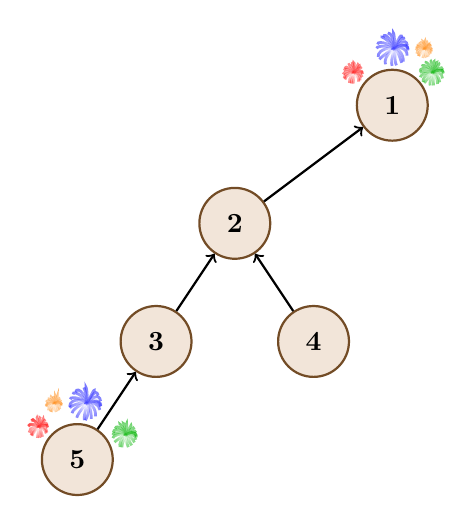
\begin{tikzpicture}[
    hobbit/.style={
      circle, draw=brown!60!black, fill=brown!20, 
      thick, minimum size=0.9cm, font=\bfseries
    },
    firework/.pic={
      \foreach \a in {0,20,...,360}{
        \draw[#1] (0,0) to [in=90] (10*rand+\a:5mm);
      }
    }
  ]

  \node[hobbit] (1) at (0,0) {1};
  \node[hobbit] (2) at (-2,-1.5) {2};
  \node[hobbit] (3) at (-3,-3) {3};
  \node[hobbit] (4) at (-1,-3) {4};
  \node[hobbit] (5) at (-4,-4.5) {5};
  
  \begin{scope}[transparency group]
    \pgfsetfading{fadein}{\pgftransformshift{\pgfpoint{0cm}{0.7cm}}}
    \pic[scale=0.4] at ($(1) + (0, 0.7)$) {firework={blue!80!white}};
    \pgfsetfading{fadein}{\pgftransformshift{\pgfpoint{-0.5cm}{0.4cm}}}
    \pic[scale=0.25] at ($(1) + (-0.5, 0.4)$) {firework={red}};
    \pgfsetfading{fadein}{\pgftransformshift{\pgfpoint{0.5cm}{0.4cm}}}
    \pic[scale=0.3] at ($(1) + (0.5, 0.4)$) {firework={green!70!black}};
    \pgfsetfading{fadein}{\pgftransformshift{\pgfpoint{0.4cm}{0.7cm}}}
    \pic[scale=0.2] at ($(1) + (0.4, 0.7)$) {firework={orange}};

    \pgfsetfading{fadein}{\pgftransformshift{\pgfpoint{-3.9cm}{-3.8cm}}}
    \pic[scale=0.4] at ($(5) + (0.1, 0.7)$) {firework={blue!80!white}};
    \pgfsetfading{fadein}{\pgftransformshift{\pgfpoint{-4.5cm}{-4.1cm}}}
    \pic[scale=0.25] at ($(5) + (-0.5, 0.4)$) {firework={red}};
    \pgfsetfading{fadein}{\pgftransformshift{\pgfpoint{-3.4cm}{-4.2cm}}}
    \pic[scale=0.3] at ($(5) + (0.6, 0.3)$) {firework={green!70!black}};
    \pgfsetfading{fadein}{\pgftransformshift{\pgfpoint{-4.3cm}{-3.8cm}}}
    \pic[scale=0.2] at ($(5) + (-0.3, 0.7)$) {firework={orange}};
  \end{scope}

  \draw[thick, ->] (2) -- (1);
  \draw[thick, ->] (3) -- (2);
  \draw[thick, ->] (4) -- (2);
  \draw[thick, ->] (5) -- (3);
\end{tikzpicture}
\end{document}
